%%=============================================================================
%% Conclusie
%%=============================================================================

\chapter{Conclusie}
\label{ch:conclusie}

%% TODO: Trek een duidelijke conclusie, in de vorm van een antwoord op de
%% onderzoeksvra(a)g(en). Wat was jouw bijdrage aan het onderzoeksdomein en
%% hoe biedt dit meerwaarde aan het vakgebied/doelgroep? Reflecteer kritisch
%% over het resultaat. Had je deze uitkomst verwacht? Zijn er zaken die nog
%% niet duidelijk zijn? Heeft het onderzoek geleid tot nieuwe vragen die
%% uitnodigen tot verder onderzoek?

\section{Snelheid}
\subsection{10 000 objecten}
Het eerste wat we gaan analyseren en een conclusie uit trekken is het verzenden van 10 000 objecten. Eerst kijken we naar de waardes apart per technologie, daarna gaan we alle technologieën gaan vergelijken met elkaar.
\subsubsection{Google Pub/Sub}
De resultaten van de snelheden bij 10 000 objecten van Google Pub/Sub zien er als volgt uit:
\begin{table}[h!]
    \centering
    \label{q1}
    \begin{tabular}{| 1 | c |}
        \hline
        & Tijd (ms)\\ \hline
        min. & 1366  \\
        gem. & 11665.7694 \\
        max. & 19365\\
        \# ontvangen. & 10 000\\ \hline
    \end{tabular}
    \caption{Verschil tussen ontvangen en verzenden (in ms) - Google Pub/Sub}
\end{table}

We zien dus dat het kleinste verschil iets meer dan één seconde is, en het grootste verschil bijna 20 seconden. Het gemiddeld aantal seconden ligt rond de 11,5 seconden.

\subsubsection{Kafka}
De resultaten van de snelheden bij 10 000 objecten van Kafka zien er als volgt uit:
\begin{table}[h!]
    \centering
    \label{q1}
    \begin{tabular}{| 1 | c |}
        \hline
        & Tijd (ms)\\ \hline
        min. & 1008  \\
        gem. & 20339.5169 \\
        max. & 38537\\
        \# ontvangen. & 10 000\\ \hline
    \end{tabular}
    \caption{Verschil tussen ontvangen en verzenden (in ms) - Kafka}
\end{table}

We zien dus dat het kleinste verschil nog dichter bij de één seconde ligt dan bij Google Pub/Sub. Het grootste verschil is bijna 40 seconden. Het gemiddeld aantal seconden ligt rond de 20 seconden.

\subsubsection{RabbitMq}
De resultaten van de snelheden bij 10 000 objecten van RabbitMq zien er als volgt uit:
\begin{table}[h!]
    \centering
    \label{q1}
    \begin{tabular}{| 1 | c |}
        \hline
        & Tijd (ms)\\ \hline
        min. & 598  \\
        gem. & 21780.9111 \\
        max. & 41805\\
        \# ontvangen. & 10 000\\ \hline
    \end{tabular}
    \caption{Verschil tussen ontvangen en verzenden (in ms) - RabbitMq}
\end{table}

Het kleinste tijdverschil is iets meer dan een halve seconde. Het grootste verschil is meer dan 40 seconden. Het gemiddeld aantal seconden is bijna 42 seconden.
\subsubsection{Vergelijking}
Om een goede vergelijking te kunnen maken tussen de drie technologieën zetten we de resultaten bij 10 000 objecten van de verschillende technologieën even naast elkaar met behulp van drie boxplots die te zien is op figuur 4.1.

 \begin{figure}[h!]
    \centering
    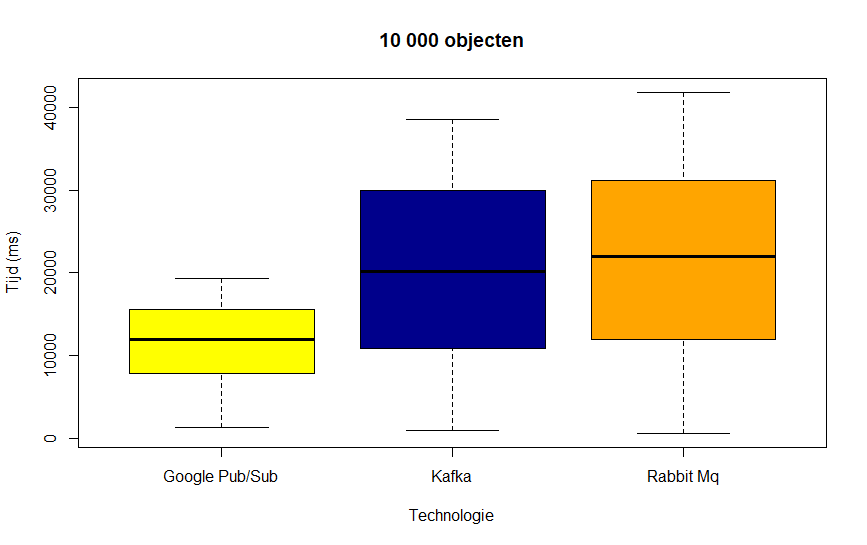
\includegraphics[width=100mm]{../10000Boxplot.png}
    \caption{Vergelijking bij 10 000 objecten}
    
\end{figure}

Bij zowel Google Pub/Sub, Kafka en RabbitMq zijn alle 10 000 objecten die verzonden zijn geweest, ook aangekomen. Dit wil zeggen dat bij 10 000 objecten geen enkel object mislukt is om te ontvangen. We kunnen bij deze hoeveelheid dus een duidelijke conclusie trekken als we kijken naar de snelheid tussen ontvangen en verzenden. 

Eerst bekijken we de minimum waarden. Daarin is te zien dat RabbitMq de kortste tijd heeft van de drie minimum waarden. Dit is dubbel zo snel als we vergelijken met Kafka, die de tweede kortste tijd heeft. RabbitMq slaagt er in om in ongeveer een halve seconde een object te verzenden en te ontvangen. Kafka doet dit slechts in één seconde. Google Pub/Sub is de slechtste leerling van de klas op het gebied van minimum tijd en doet er ongeveer 1,3 seconden over.

Laat ons nu kijken naar de maximum tijd. Hier doet Google Pub/Sub het veruit beter of de twee andere technologieën. Het doet er nooit langer dan 20 seconden over om een bericht te versturen en weer te lezen. Hier doen Kafka en RabbitMq het veel slechter. Zij doen er maximum 3,8 en 4,1 seconde over, en dit is veel meer of bij Google Pub/Sub.

Het resultaat van de maxima weerspiegelt zich ook in de gemiddeldes. Gemiddeld doet Google Pub/Sub er 11 seconden over. Het gemiddelde van Kafka en RabbitMq ligt dan weer wat hoger met 20 en 21 seconden.

Conclusie bij 10 000 objecten: Alhoewel de minimum tijd bij Google Pub/Sub hoger ligt of bij Kafka en RabbitMq, slaagt Google Pub/Sub er toch in om behoorlijk wat sneller al de data te verwerken. 


\subsection{100 000 objecten}
Het lijkt ons ook interessant om eens te bekijken wat te resultaten zijn indien we het aantal objecten wat gaan verhogen. We nemen tien keer zo veel objecten en kijken wat we hiermee kunnen uit concluderen.
\subsubsection{Google Pub/Sub}
De resultaten van de snelheden bij 100 000 objecten van Google Pub/Sub zien er als volgt uit:
\begin{table}[h!]
    \centering
    \label{q1}
    \begin{tabular}{| 1 | c |}
        \hline
        & Tijd (ms)\\ \hline
        min. &  1753\\
        gem. & 88603.80396 \\
        max. & 169580\\
        \# ontvangen. & 100 000\\ \hline
    \end{tabular}
    \caption{Verschil tussen ontvangen en verzenden (in ms) - Google Pub/Sub}
\end{table}

We zien dus dat het kleinste verschil iets minder is dan twee seconden, en het grootste verschil bijna 170 seconden, wat bijna drie minuten is. Het gemiddeld aantal seconden ligt rond de 88 seconden, wat bijna 1,5 minuten is.

\subsubsection{Kafka}
De resultaten van de snelheden bij 100 000 objecten van Kafka zien er als volgt uit:
\begin{table}[h!]
    \centering
    \label{q1}
    \begin{tabular}{| 1 | c |}
        \hline
        & Tijd (ms)\\ \hline
        min. & 1055  \\
        gem. & 175526.39283 \\
        max. & 346431\\
        \# ontvangen. & 100 000\\ \hline
    \end{tabular}
    \caption{Verschil tussen ontvangen en verzenden (in ms) - Kafka}
\end{table}

Het kleinste verschil blijft nog steeds dicht bij de één seconde liggen, alhoewel het verschil toch lichtjes gestegen is. Het grootste verschil ligt rond de 346 seconden, wat bijna zes minuten is. Het gemiddeld aantal seconden ligt rond de 175 seconden, omgerekend is dit bijna drie minuten.

\subsubsection{RabbitMq}
De resultaten van de snelheden bij 100 000 objecten van RabbitMq zien er als volgt uit:
\begin{table}[h!]
    \centering
    \label{q1}
    \begin{tabular}{| 1 | c |}
        \hline
        & Tijd (ms)\\ \hline
        min. & 458  \\
        gem. & 114365.12135045651 \\
        max. & 224467\\
        \# ontvangen. & 59 802\\ \hline
    \end{tabular}
    \caption{Verschil tussen ontvangen en verzenden (in ms) - RabbitMq}
\end{table}

Wat meteen opvalt, is dat bij deze hoeveelheid RabbitMq er niet in geslaagd is om tijdens dezelfde run alle 100 000 objecten binnen te halen. Natuurlijk haalt hij deze wel nog binnen indien de applicatie opnieuw opgestart wordt, maar het is toch opvallend dat maar iets meer of de helft meteen ontvangen wordt.

De minimum tijd is nog gedaald in vergelijking met 10 000 objecten. Hij heeft nu slechts minder dan een halve seconde nodig om te verzenden en te ontvangen. Het gemiddelde ligt rond de 114 seconden en het maximum iets meer dan 224 seconden. Natuurlijk zijn het gemiddelde en maximum minder belangrijk om te vergelijken aangezien niet alle 100 000 objecten zijn ontvangen.
\subsubsection{Vergelijking}
Ook bij deze hoeveelheid aan objecten zetten we de drie technologieën eens naast elkaar. Deze boxplots zijn te zien op figuur 4.2

\begin{figure}[h!]
    \centering
    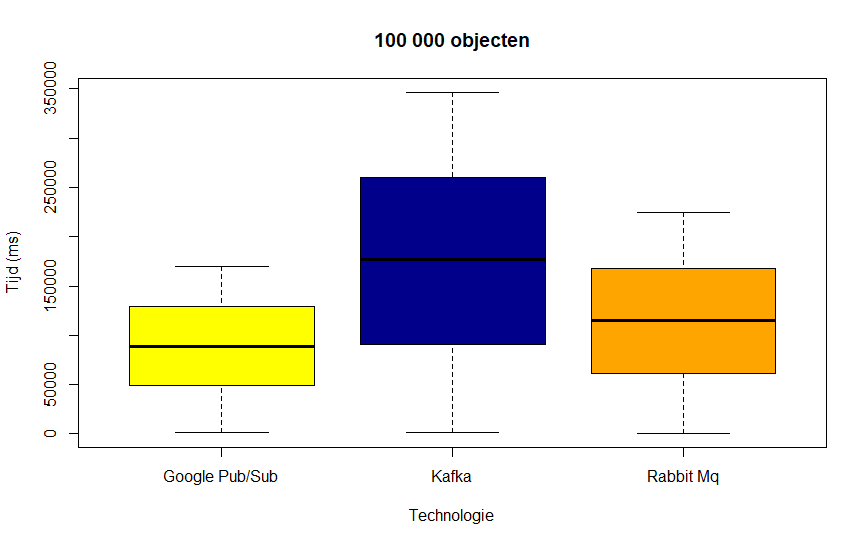
\includegraphics[width=100mm]{../100000Boxplot.png}
    \caption{Vergelijking bij 100 000 objecten}
    
\end{figure}

Hierbij is het minder relevant om RabbitMq helemaal te gaan vergelijken met de twee andere technologieën aangezien maar iets meer dan de helft van de objecten ook ontvangen zijn geweest.

Eerst gaan we de minimum waarden bekijken, hier kunnen we ook nog vergelijken met RabbitMq. Daarin is te zien dat RabbitMq de kortste tijd heeft van de drie minimum waarden. Deze waarde is zelf nog minder dan bij de vorige vergelijking van 10 000 objecten. Kafka blijft redelijk stabiel van de kortste tijd en schommelt nog steeds rond de seconde. Bij Google Pub/Sub zien we toch een stijging en deze waarde is nu 1,7 seconden geworden.

Laat ons nu kijken naar de maximum tijd. Hier doet opnieuw Google Pub/Sub het veruit beter of de twee andere technologieën. We zouden kunnen zeggen dat de waarde bij RabbitMq ook nog goed meevalt, maar dit zou een vertekend beeld geven omdat niet alle objecten ontvangen zijn geweest. Dus het heeft enkel zin om voor de maximum waarde Google Pub/Sub te gaan vergelijken met Kafka. Bij Kafka ligt de maximum waarde veel hoger. Het heeft er maximum ongeveer 346 seconden voor nodig, wat bijna dubbel zo veel is dan bij Google Pub/Sub.

Het resultaat van de maxima weerspiegelt zich ook opnieuw in de gemiddeldes. Ook hier houden we geen rekening met RabbitMq want niet alle objecten zijn ontvangen. We kunnen eigenlijk al zeker concluderen dat bij 100 000 objecten Google Pub/Sub sowieso sneller zou geweest zijn dan RabbitMq aangezien het gemiddelde voor minder ontvangen waarden al hoger ligt dan bij Google Pub/Sub. Gemiddeld doet Google Pub/Sub er 88 seconden over. Het gemiddelde van Kafka ligt dan weer wat hoger met 175 seconden.

Conclusie bij 100 000 objecten: Alhoewel de minimum tijd bij Google Pub/Sub opnieuw hoger ligt of bij Kafka en RabbitMq, slaagt Google Pub/Sub er toch in om behoorlijk wat sneller al de data te verwerken. 

\subsection{1 000 000 objecten}
De laatste hoeveelheid objecten die we onderzoeken is nog eens tien keer zo veel. We kijken ook eens wat het resultaat is bij 1 000 000 objecten.
\subsubsection{Google Pub/Sub}
De resultaten van de snelheden bij 1 000 000 objecten van Google Pub/Sub zien er als volgt uit:
\begin{table}[h!]
    \centering
    \label{q1}
    \begin{tabular}{| 1 | c |}
        \hline
        & Tijd (ms)\\ \hline
        min. &  3327\\
        gem. & 577596.5258098603 \\
        max. & 1037761\\
        \# ontvangen. & 556 454\\ \hline
    \end{tabular}
    \caption{Verschil tussen ontvangen en verzenden (in ms) - Google Pub/Sub}
\end{table}

We zien dus dat het kleinste verschil iets meer is dan drie seconden, en het grootste verschil bijna 1037 seconden, wat bijna 17 minuten is. Het gemiddeld aantal seconden ligt rond de 577 seconden, wat iets meer dan 9,5 minuten is. Hier is Google Pub/Sub voor het eerst niet in geslaagd om alle objecten te ontvangen. Het zal dus ook hier wat moeilijker zijn om het gemiddelde en het maximum te vergelijken.

\subsubsection{Kafka}
De resultaten van de snelheden bij 1 000 000 objecten van Kafka zien er als volgt uit:
\begin{table}[h!]
    \centering
    \label{q1}
    \begin{tabular}{| 1 | c |}
        \hline
        & Tijd (ms)\\ \hline
        min. & 3930  \\
        gem. & 1719014.245389 \\
        max. & 3424980\\
        \# ontvangen. & 1 000 000\\ \hline
    \end{tabular}
    \caption{Verschil tussen ontvangen en verzenden (in ms) - Kafka}
\end{table}

Het kleinste verschil ligt nu niet meer rond de seconde, maar is nu gestegen naar bijna vier seconden. Het grootste verschil ligt rond de 3424 seconden, wat bijna een uur is. Het gemiddeld aantal seconden ligt rond de 1719 seconden, omgerekend is dit bijna een half uur.

\subsubsection{RabbitMq}
De resultaten van de snelheden bij 1 000 000 objecten van RabbitMq zien er als volgt uit:
\begin{table}[h!]
    \centering
    \label{q1}
    \begin{tabular}{| 1 | c |}
        \hline
        & Tijd (ms)\\ \hline
        min. & 1345  \\
        gem. & 300640.46033216227 \\
        max. & 590104\\
        \# ontvangen. & 59 802\\ \hline
    \end{tabular}
    \caption{Verschil tussen ontvangen en verzenden (in ms) - RabbitMq}
\end{table}

RabbitMq is ook hier niet in geslaagd om alle objecten te ontvangen. De minimum tijd is voor het eerst gestegen naar iets meer dan een seconde. Het gemiddelde ligt op 300 seconden. En het duurt nooit langer dan 590 seconden of een kleine tien minuten om een object te ontvangen.

\subsubsection{Vergelijking}
Ook bij deze hoeveelheid aan objecten zetten we de drie technologieën eens naast elkaar. Deze boxplots zijn te zien op figuur 4.3

\begin{figure}[h!]
    \centering
    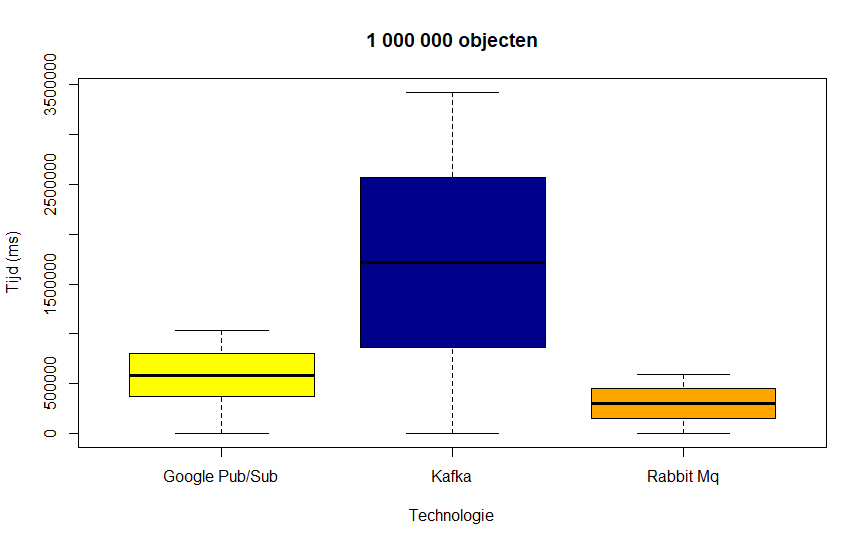
\includegraphics[width=100mm]{../1000000Boxplot.png}
    \caption{Vergelijking bij 1 000 000 objecten}
    
\end{figure}

Nu is het wat moeilijker om de snelheden met elkaar te gaan vergelijken aangezien de drie verschillende technologiëen verschillend aantal objecten hebben ontvangen. Toch overlopen we de technologieën eens.

Eerst gaan we de minimum waarden bekijken, hier kunnen we nog alle drie met elkaar vergelijken. Daarin is te zien dat RabbitMq nog steeds de kortste tijd heeft van de drie minimum waarden. Deze waarde is wel gestegen naar iets boven de seconde, maar blijft nog steeds de beste. Kafka is voor het eerst ook opvallend gestegen. De waarde is bijna vier keer zo groot geworden. Bij Google Pub/Sub zien we ook een stijging, het minimum ligt nu ook rond de drie seconden. Kafka heeft dus bij deze hoeveelheid het meeste tijd nodig als minimum waarde. 

Laat ons nu kijken naar de maximum tijd. Dit is wat moeilijker om te vergelijken aangezien al de technologieën verschillend aantal objecten ontvangen hebben. Kafka heeft het meeste tijd nodig, maar heeft ook het meeste objecten ontvangen. RabbitMq en Google Pub/Sub hebben ongeveer evenveel ontvangen, en daar zien we RabbitMq toch duidelijk beter zijn voor de maximum waarde.

Het resultaat van de maxima weerspiegelt zich ook opnieuw in de gemiddeldes. De verhoudingen zijn hetzelfde als bij de maximum waardes

Conclusie bij 1 000 000 objecten: RabbitMq doet het beter dan Google Pub/Sub. Kafka is moeilijk te vergelijken met de twee andere.

\subsection{Conclusie snelheid}
Op het gebied van snelheid is Kafka over het algemeen gezien de slechtste. Google Pub/Sub doet het over het algemeen gezien het beste, behalve bij super veel objecten (hier: 1 000 000) doet RabbitMq beter dan Google Pub/Sub.

\section{Memory}
\subsection{1 000 objecten}
Omdat de operatie om aan de Java runtime de gebruikte memory te vragen te lang duurt, wordt er enkel gekeken bij 1 000 objecten. Er wordt hier geen rekening gehouden met de snelheden.
\subsection{Conclusie memory}

Op figuur 4.4 ziet u de boxplots van het resultaat van het memory gebruik. Het is duidelijk te zien dat er bij alle technologieën enkele uitschieters zijn. Maar het is ook duidelijk dat over het algemeen voor het memory gebruik RabbitMq beter is. Het gemiddelde, maximum en het minimum liggen lager in vergelijking met de andere. Gemiddeld heeft RabbitMq 33.138 MB nodig. Google Pub/Sub en Kafka hebben gemiddeld 36.31 en 33.601 nodig. RabbitMq is dus beter maar het verschil met Kafka is klein. Het is enkel Google Pub/Sub die veel meer memory nodig heeft dan de rest.
\begin{figure}[h!]
    \centering
    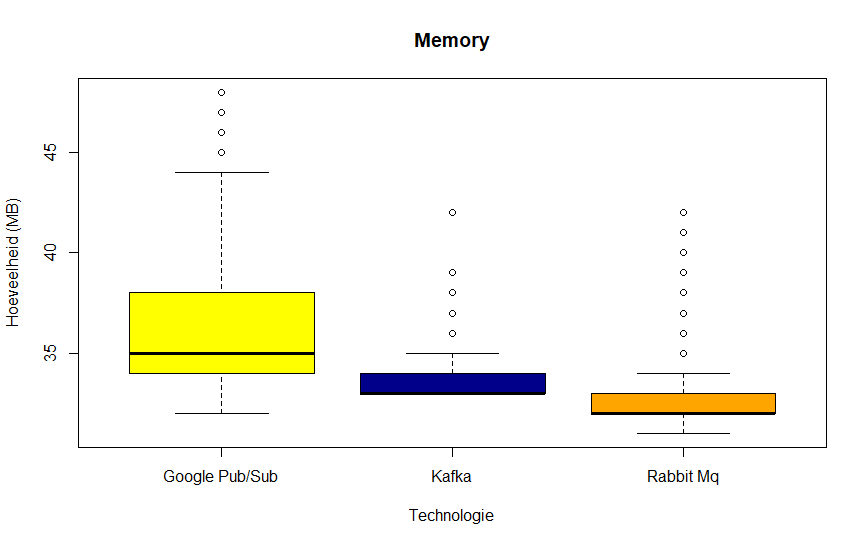
\includegraphics[width=100mm]{../memory.png}
    \caption{Vergelijking memory}
    
\end{figure}



\section{Algemene conclusie}
Wanneer snelheid voor een bedrijf het belangrijkste is, dan lijkt Google Pub/Sub het beste. Tenzij je heel veel objecten hebt (meer dan 1 000 000) dan lijkt RabbitMq sneller te werken. Het memory gebruik is het best bij RabbitMq maar Kafka doet het niet veel slechter. Bij Kafka ben je het meest zeker dat je effectief al je verzonden data meteen ontvangt. Hier slaagt RabbitMq het slechtste op.

Voor TVH specifiek lijkt het belangrijkste dat alle data zeker meteen ontvangen wordt. Omdat Kafka hierop het beste scoort en bijna de beste is op basis van memory gebruik, lijkt Kafka de beste technologie om te gebruiken binnen dit bedrijf.

Een verder onderzoek zou dit onderzoek enkele keren kunnen herhalen om te bepalen hoe frequent verzonden data niet meteen aankomt. Ook zouden we de applicaties in een ander onderzoek in de cloud kunnen laten draaien zodat deze niet afhankelijk zijn van een lokale pc of laptop.

